%%%%%%%%%%%%%%%%%%%%%%%%%%%%%%%%%%%%%%%%%
% Short Sectioned Assignment
% LaTeX Template
% Version 1.0 (5/5/12)
%
% This template has been downloaded from:
% http://www.LaTeXTemplates.com
%
% Original author:
% Frits Wenneker (http://www.howtotex.com)
%
% License:
% CC BY-NC-SA 3.0 (http://creativecommons.org/licenses/by-nc-sa/3.0/)
%
%%%%%%%%%%%%%%%%%%%%%%%%%%%%%%%%%%%%%%%%%

%----------------------------------------------------------------------------------------
%	PACKAGES AND OTHER DOCUMENT CONFIGURATIONS
%----------------------------------------------------------------------------------------

\documentclass[paper=a4, fontsize=11pt]{scrartcl} % A4 paper and 11pt font size
\usepackage[a4paper,
			bottom=1.5in,
			left=1.2in,
			right=1.2in,
			top=1.2in,
			headsep = 35pt]
	{geometry}
\usepackage[T1]{fontenc} % Use 8-bit encoding that has 256 glyphs
\usepackage{fourier} % Use the Adobe Utopia font for the document - comment this line to return to the LaTeX default

\usepackage[english]{babel} % English language/hyphenation
%\usepackage[ngerman]{babel}
\usepackage{amsmath,amsfonts,amsthm} % Math packages

\usepackage{lipsum} % Used for inserting dummy 'Lorem ipsum' text into the template

\usepackage{sectsty} % Allows customizing section commands
\allsectionsfont{\centering \normalfont\scshape} % Make all sections centered, the default font and small caps

\usepackage{fancyhdr} % Custom headers and footers
\pagestyle{fancyplain} % Makes all pages in the document conform to the custom headers and footers
\fancyhead{} % No page header - if you want one, create it in the same way as the footers below
\fancyfoot[L]{} % Empty left footer
\fancyfoot[C]{} % Empty center footer
\fancyfoot[R]{\thepage} % Page numbering for right footer
\renewcommand{\headrulewidth}{0pt} % Remove header underlines
\renewcommand{\footrulewidth}{0pt} % Remove footer underlines
\setlength{\headheight}{13.6pt} % Customize the height of the header

\numberwithin{equation}{section} % Number equations within sections (i.e. 1.1, 1.2, 2.1, 2.2 instead of 1, 2, 3, 4)
\numberwithin{figure}{section} % Number figures within sections (i.e. 1.1, 1.2, 2.1, 2.2 instead of 1, 2, 3, 4)
\numberwithin{table}{section} % Number tables within sections (i.e. 1.1, 1.2, 2.1, 2.2 instead of 1, 2, 3, 4)

%\setlength\parindent{0pt} % Removes all indentation from paragraphs - comment this line for an assignment with lots of text

\usepackage[utf8]{inputenc} %damit Umlaute gehen
%\usepackage{hyperref} %Verlinkungen ins Inhaltsverzeichnis
\usepackage{amsmath} %Required for Math symbols
\usepackage{amssymb}
\usepackage{listings} % Required for insertion of code

\usepackage[usenames,dvipsnames]{color} % Required for custom colors
\usepackage{graphicx} % Required to insert images

\usepackage{booktabs} % Allows the use of \toprule, \midrule and \bottomrule in tables for horizontal lines

\usepackage{caption} %Zeilenumbruch in Bildbeschreibung
\captionsetup{
  format=hang,
  justification=centering,
  singlelinecheck=off
}

%\usepackage[tocflat]{tocstyle}
%\usetocstyle{standard}

\usepackage{tocloft}% http://ctan.org/pkg/tocloft
\renewcommand{\cftsecfont}{}
\renewcommand{\cftsecpagefont}{}

\usepackage{float}
\usepackage{url}

\DeclareOldFontCommand{\bf}{\normalfont\bfseries}{\mathbf}

%\usepackage{mathabx}
\usepackage{amsmath}

%----------------------------------------------------------------------------------------
%	CODE INCLUSION CONFIGURATION
%----------------------------------------------------------------------------------------

\definecolor{MyDarkGreen}{rgb}{0.0,0.4,0.0} % This is the color used for comments
\lstloadlanguages{Matlab} % Load Perl syntax for listings, for a list of other languages supported see: ftp://ftp.tex.ac.uk/tex-archive/macros/latex/contrib/listings/listings.pdf
\lstset{language=Matlab, % Use Perl in this example
        frame=single, % Single frame around code
        basicstyle=\small\ttfamily, % Use small true type font
        keywordstyle=[1]\color{Blue}\bf, % Perl functions bold and blue
        keywordstyle=[2]\color{Purple}, % Perl function arguments purple
        keywordstyle=[3]\color{Blue}\underbar, % Custom functions underlined and blue
        identifierstyle=, % Nothing special about identifiers
        commentstyle=\usefont{T1}{pcr}{m}{sl}\color{MyDarkGreen}\small, % Comments small dark green courier font
        stringstyle=\color{Purple}, % Strings are purple
        showstringspaces=false, % Don't put marks in string spaces
        tabsize=5, % 5 spaces per tab
        %
        % Put standard Perl functions not included in the default language here
        morekeywords={rand},
        %
        % Put Perl function parameters here
        morekeywords=[2]{on, off, interp},
        %
        % Put user defined functions here
        morekeywords=[3]{test},
       	%
        morecomment=[l][\color{Blue}]{...}, % Line continuation (...) like blue comment
        numbers=left, % Line numbers on left
        firstnumber=1, % Line numbers start with line 1
        numberstyle=\tiny\color{Blue}, % Line numbers are blue and small
        stepnumber=5, % Line numbers go in steps of 5
				literate=%
					{Ö}{{\"O}}1
					{Ä}{{\"A}}1
					{Ü}{{\"U}}1
					{ß}{{\ss}}2
					{ü}{{\"u}}1
					{ä}{{\"a}}1
					{ö}{{\"o}}1
}

% Creates a new command to include a perl script, the first parameter is the filename of the script (without .pl), the second parameter is the caption
\newcommand{\matlabscript}[2]{
\begin{itemize}
\item[]\lstinputlisting[caption=#2,label=#1]{#1.m}
\end{itemize}
}


%----------------------------------------------------------------------------------------
%	TITLE SECTION
%----------------------------------------------------------------------------------------

\newcommand{\horrule}[1]{\rule{\linewidth}{#1}} % Create horizontal rule command with 1 argument of height

\title{
\normalfont \normalsize
\textsc{Technical University Vienna, SEM Machine Learning} \\ [25pt] % Your university, school and/or department name(s)
\horrule{0.5pt} \\[0.4cm] % Thin top horizontal rule
\huge Introduction to Reinforcement Learning: Multiarmed Bandit Problem, Finite MDPs  \\ % The assignment title
\horrule{2pt} \\[0.5cm] % Thick bottom horizontal rule
}

\author{Felix Wagner, Matr.nr. 01426449, mailfwagner@gmail.com} % Your name

\date{\normalsize\today} % Today's date or a custom date

\begin{document}

\maketitle % Print the title

%----------------------------------------------------------------------------------------
%	PROBLEM 1
%----------------------------------------------------------------------------------------

\section*{Abstract}

	Reinforcement Learning is one of the three big areas in Machine Learning. It's objective is finding optimal strategies to solve a given problem. In this paper the basics of Reinforcement Learning are explained and the content is applied to a generic project.

	In the first chapter, the definition of an agent and his environment, actions and rewards is introduced. Some basic assumptions about the agents policy of decision making and the importance of exploration and exploitation are explained. A walk-through of a first example, winning a Tic-Tac-Toe game, is given.

	The second chapter compares different methods to find an optimal policy heuristically, by the example of the Multiarmed-Bandit-Problem. Especially the $\epsilon$-greedy method is presented.

	The third chapter deals with a more rigorous mathematical framework for modeling Reinforcement Learning problems, namely Finite Markov Decision Processes. The Bellman Equation, as well as the Bellman Optimality Equation and the value of different states and state-action pairs are introduced. The state values of different policies for the game Gridworld are calculated.

	The fourth and last chapter walks through a small project: Finding the best way of escaping a labyrinth. The results are discussed, as well as possible improvements.
 

\section{Introduction}

\subsection{Categorization of Machine Learning}

	Machine Learning Problems can generally be categorized into three classes: 
\begin{itemize}
\item Supervised Learning: Typically classification or regression problems, for which a lot of labeled data is available. The following would be a classification problem: There are 5000 pictures given, and it is known which of them shows a cat. The algorithm shall learn to recognize cats on other pictures as well. Whereas the following would be a regression problem: The properties and prices of 1000 houses in Vienna are given, the algorithm shall predict the prices of other houses in Vienna, according to their properties. 
\item Unsupervised Learning: A lot of data is available, but it is not labeled. The algorithm shall find some underlying structure. Despite this class seems way more open-ended, it is often used for data compression. By summarizing the features of given data, the relevant parts can be extracted and therefore processed and stored more efficiently. 
\item Reinforcement Learning (RL): This class does not deal with data at all, but with a given problem in decision making. A typical problem would be: Find the best strategy to win a game of chess. The game is then modeled as an optimization problem, in which a fictive player (agent) gets points (rewards) for smart moves and the other way around. Then the algorithm tries to get as much points as possible, over a given time period.
\end{itemize}

	In this paper only with the third class, Reinforcement Learning (RL), will be dealt. In applications, very often all three are applied together. For instance in cost-intensive RL problems, many functions are computed as neural networks, which themselves fall into the class of supervised learning.

\subsection{Agent-Environment Interaction}

	Every RL problem can be thought of in the following way: An agent  is surrounded by an environment. The environment is in a certain state and the agent can set certain actions. When the agent sets an action, the state of the environment may change and the agent may obtain a reward, which is a scalar numerical value. All those depend on each other: The actions the agent may set depend on the state, as well as the reward the agent obtains for his action. The change of the state also depends on the action and the former state. This builds a trajectory of states, actions and rewards, like it is pictured in \ref{fig:agentenv}. 

\begin{figure}[H]
\centering
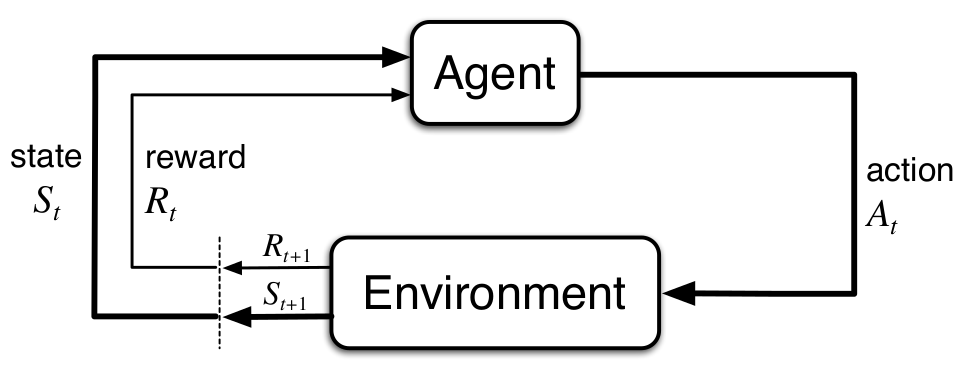
\includegraphics[width=0.6\columnwidth]{Images/AgentEnvironment.png}
\caption{ \cite{SuttonBarto} The Interaction of agent and environment build a trajectory of states, actions and rewards at different time steps: $S_0 \rightarrow A_0 \rightarrow \{ R_{1}, S_1 \} \rightarrow A_1 \rightarrow \{ R_{2}, S_2 \} \rightarrow A_2 ...$}
\label{fig:agentenv}
\end{figure}

	The objective of the agent is to maximize the rewards over time.  The immediate reward on an action contains no information about the expected future rewards in the new state. This means, the agent has to find a strategy to estimate those future rewards.

\subsection{Policies and Values}

	The agent sets his actions according to a function, called policy $\pi$. This policy depends on the current state $s$ of the environment. A policy can be deterministic, which means it maps the state $s$ to an action $a$: $s \mapsto a$; But usually policies are stochastic, that means it maps a state $s$ and an action $a$ to a probability $p$ of taking that action: $(a|s) \mapsto p$. A policy that leads to expected future rewards that are greater than or equal to those of all other policies, for every state, is called an optimal policy $\pi_*$.

	In the process of finding an optimal policy, there are often values assigned to certain states or state-action pairs. For that sake, the value function $v_\pi(s)$ assigns a single numerical value to every state, and the action-value function $q_\pi(a|s)$ to every state-action pair. Ideally the values should be proportional to the expected future rewards. 

	There are various strategies to arrive at an optimal policy, but all of them have to balance two essential phases: Exploration and Exploitation. The agent does not know the reactions of the environment to an action, until he gave it a try. So when the agent starts the problem, he has to try a lot of different actions in a lot of different states, to get an idea of his possibilities. This phase is called exploration and the agent may not place importance on high rewards in this phase. This behavior would risk him not finding other paths of the problem, which lead to even higher rewards. Usually this is the phase where the agent assigns somewhat meaningful values to the states and actions, to remember for later moves, which paths are worthwhile. When the agent has enough values assigned, he can start exploiting. In this phase he follows mainly the highest values of actions and states, relying on the exploration he did before. If the first phase was done properly, the agent should have found an optimal policy by just following the highest values. In applications, those phases will usually not be strictly separated. The agent will rather alternate between explorative and exploitative moves.

\subsection{Winning Tic-Tac-Toe}

	To give a first and simple example of the process of Reinforcement Learning, an optimal policy to winning Tic-Tac-Toe will now be found. The game is played by two players on a 3 times 3 fields board. In the beginning the board is empty and the players alternatingly set stones of two different colors on the board. The player who has at first three stones in a row, wins. The game is very simple as is contains maximal 9 time steps. In our RL-model, the position of all stones on the board is the current state and the state, together with the opposite player, is the environment. As on every field sits either a stone of one or the other color, or it is empty, there are $3^9 = 19683$ different possible states. At first a value function is initialized, by assigning the value $1$ to all states where the agent has three stones in a row and therefore won, and $0$ to all states where the opposite player has three stones in a row. All other states are initialized to $0.5$. 

	Now the agent has to start playing against his opponent. For that, he follows a so-called $\epsilon$-greedy strategy: At every time step he takes with probability $\epsilon$ an explorative move, which in this case means an uniformly random move, with no respect to the values. With probability $1-\epsilon$ he takes the so called greedy move, which leads him to the state with the highest reachable value. If two reachable states have the same value, the agent chooses again randomly between them. 

	The agent wants the value function, and therefore the policy, to improve with every time step. For that, an update rule is applied to the value function: After every greedy move, the value $v(s_t)$ of a state $s_t$ at time step $t$  is overwritten by a new value 

\begin{align}
v(s_t) \leftarrow v(s_t) + \alpha[v(s_{t+1}) - v(s_{t})].
\end{align}

	Here $\alpha \in [0,1]$ is a numerical parameter, called the learning rate or sometimes stepsize parameter. The update rule moves the values of consecutive states closer together and therefore raises the value of states, from which it is more likely to win, and lowers the value of states, which more likely lead to a defeat. 

	If the learning rate is lowered over time, the values of the states converge towards the real probabilities of winning from a certain state. It should be mentioned, that this example uses no rewards or action values. Furthermore, as Tic-Tac-Toe is a very easy game. It is very simple, also for a human player, to find an optimal policy, by which every round ends either in a win or in a draw. If the opponent follows this optimal policy from the beginning and therefore the agent never wins, the agent has no opportunity to find the $1$-valued states and will never find a optimal policy himself. Nevertheless, he will find a policy to avoid defeats and always reach a draw. 

\subsection{Remark about Complex Real World Problems}

	All RL problems make use of the so called Reward Hypothesis. It states, that everything that one can achieve, can be described as maximization of a single numerical value. This hypothesis holds for most problems in engineering. It gets more difficult if one thinks about more complex tasks, like human decision making. To model all decisions of a human person in a RL fashion, this persons life would only consist of the maximization of pleasure. Most humans might agree, that life is often more complex than that, starting by ethical considerations and consequently leading up to the multiple and often controversial emotions, by which nearly every human is driven. 

\section{Multi Armed Bandit Problem}

	A Multi Armed Bandit is a Slot machine with multiple levers, which can be found in Casinos and gambling houses. We will discuss two different ways to arrive at an optimal policy for playing at a Ten Armed Bandit. Every of the ten arms corresponds to an action, and the Bandit does not change it's observable state at all. So the agent is always confronted with the same state and the same 10 possible actions. We assume furthermore, that the reward distribution for every action is static, i.e. does not change over time. This example is simulated in \cite{SuttonBarto} and on ShangtongZhang's GitHub account\cite{ShangtongZhang}. The distribution of the reward of every action is shown in Fig. \ref{fig:rewarddist}. The action value $q_t(a)$ of an action $a$ can now be estimated by the rule:

\begin{align}
q_t(a) = \frac{ \sum_{i=0}^n R_i}{n}
\label{eq:estactval}
\end{align}

	Here $R_i$ denotes the reward that was obtained in time step $i$ and $n$ the number of times $a$ was taken prior to $t$.

\begin{figure}[H]
\centering
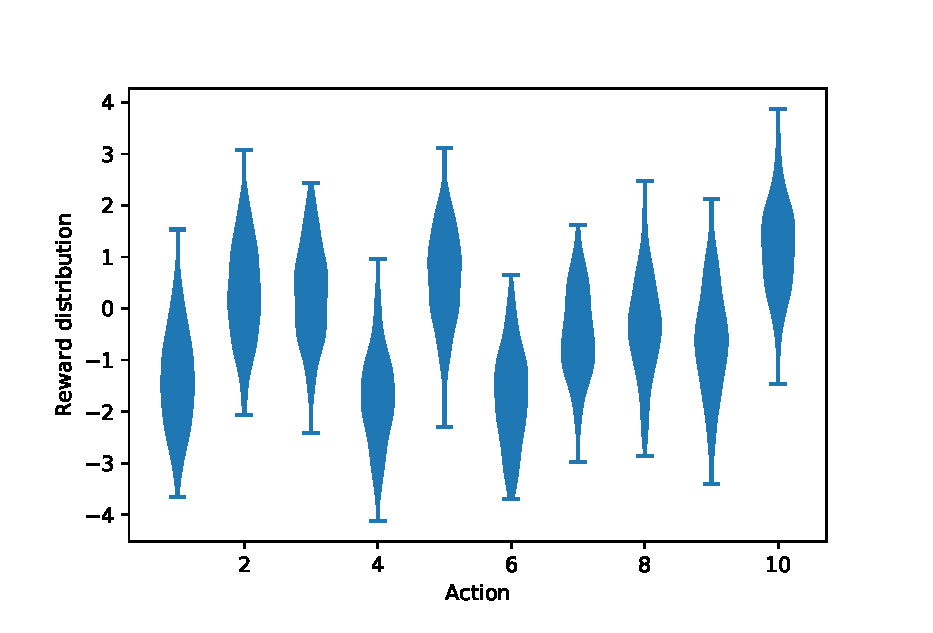
\includegraphics[width=0.6\linewidth]{Images/figure_2_1.eps}
\caption{\cite{ShangtongZhang} The rewards for every action are normally distributed and their expactations $\mu_i$ equal the real action values $q_{i,*}$, with a standard deviation of $\sigma_i = 1$. The real action values themselves are also normally distributed with expactation $\mu = 0$ and standard deviation $\sigma = 1$.}
\label{fig:rewarddist}
\end{figure}

\subsection{$\epsilon$-greedy Method}

	The first algorithm to arrive at an optimal policy is the $\epsilon$-greedy method, that was already discussed beforehand. It is a very simple method, nevertheless it builds the basis for a variety of other, more complex procedures and is therefore very important. The algorithm works as it is shown here:

\begin{lstlisting}
Set up a table with initial estimations for every action value
Choose epsilon between 0 and 1
For every time step:
	with probability epsilon: take a random non-greedy action
	else: take a greedy action and update the value
\end{lstlisting}

	The estimations of the action values can be updated by the following rule, and still satisfy equation \ref{eq:estactval}:	
	
\begin{align}
 q_{n+1} = q_n + \frac{1}{n} \big[ R_n - q_n \big] 
\end{align}

	Here $q_n$ denotes the action value at the $n$'th time step and $r_n$ the obtained reward at the $n$'th time step. 

	This was implemented in \cite{SuttonBarto}, \cite{ShangtongZhang}. The learning curve for different values of $\epsilon$ and for the first 1000 time steps is shown in Fig. \ref{fig:epsilongreedy}. For smaller $\epsilon$, the agent explores less and therefore starts off by using the greedy actions all the time. This seemingly is the best strategy throughout the first 50 to 100 time steps, but then the agents that also explore, not only exploit, reach far higher average rewards. It seems like a peak is reached somewhere around an average reward of $1.4$. 

\begin{figure}[H]
\centering
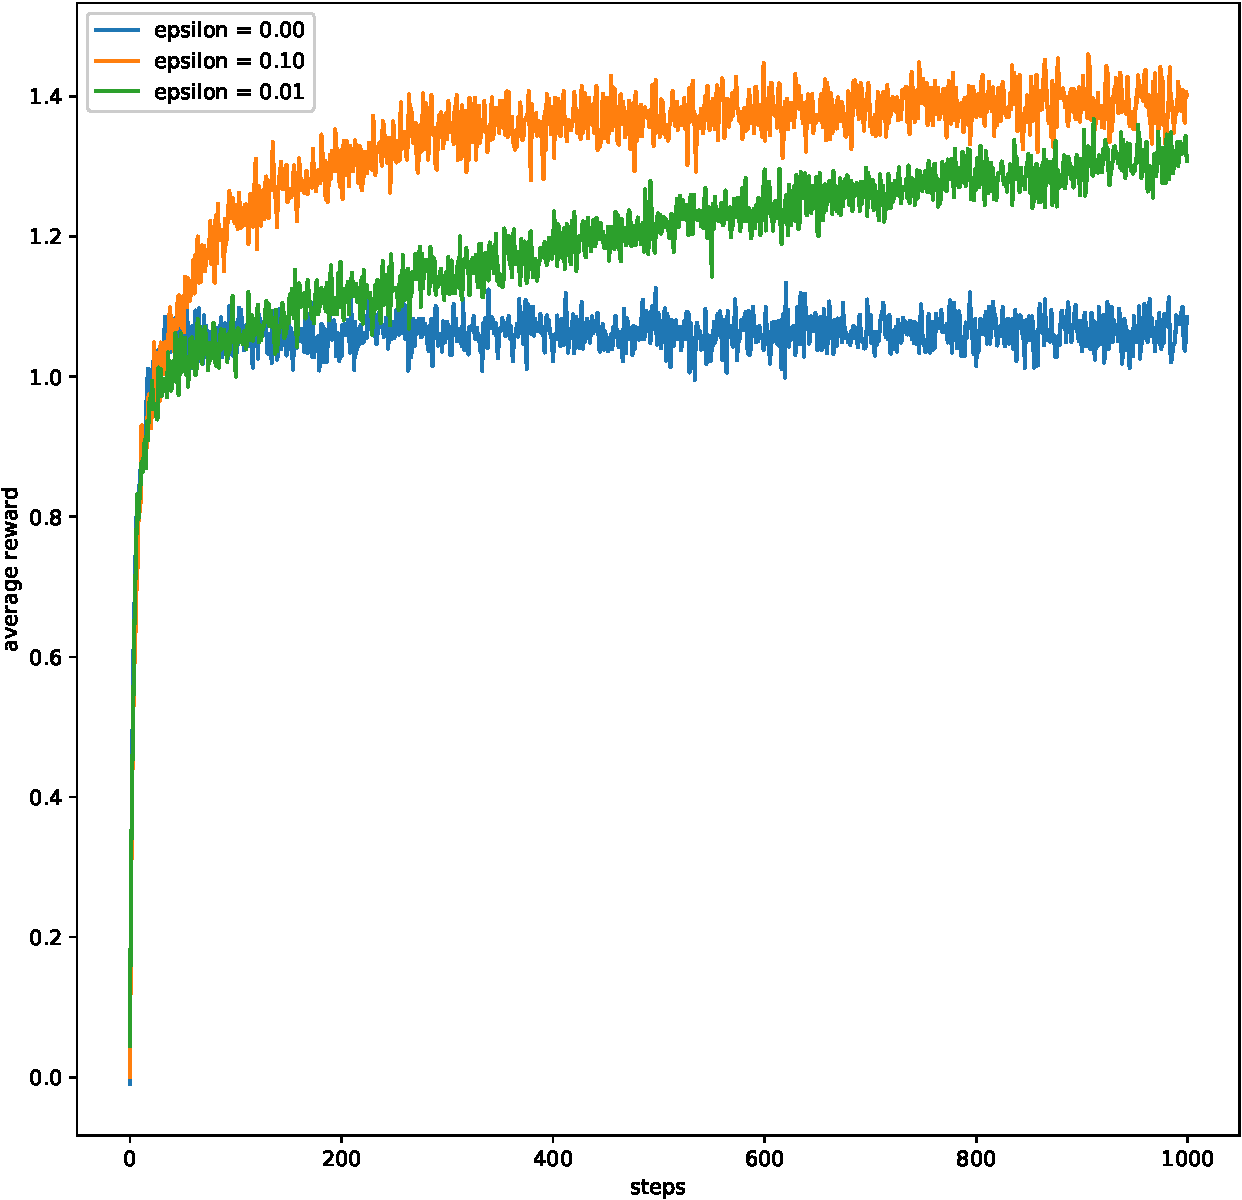
\includegraphics[width=0.6\linewidth]{Images/figure_2_2_a-crop.pdf}
\caption{\cite{ShangtongZhang} Average rewards of the $\epsilon$-greedy method, for different values of $\epsilon$ and the first 1000 time steps. It can be seen, that the blue line, which corresponds to $\epsilon = 0$, has the highest average rewards in the first 50 to 100 time steps.}
\label{fig:epsilongreedy}
\end{figure}

\subsection{Upper Confidence Bound Action Selection}

	While classifying actions as either greedy or non-greedy can be considered a coarse classification, the UCB Action Selection distiguishes subtler. The selection between non-greedy actions depends on two variables: How close is the estimate of the action to beeing greedy? And how much uncertainty is in those estimates? The rule is formulated as follows:

\begin{align}
a_t = arg \max\limits_{a}  \big[ Q_t (a) + c \sqrt{\frac{ln (t)}{N_t (a)}} \big]
\end{align}

	Here $N_t(a)$ is the number of times $a$ was selected prior to time step $t$, $c > 0$ controls the degree of exploration and if $N_t(a) = 0$, then $a$ is considered to be an maximizing action. $a_t$ is then the action which will be taken at time step $t$. This forces the agent to choose rarely used actions more often, and actions with an higher estimate also more often. The performance of this method is shown in Fig. \ref{fig:UCB}, and visibly exceeds the performance of the $\epsilon$-greedy method after 300 time steps. The spikes in the first 20 time steps are probably due to the actions that were not yet chosen and therefore produce a singularity in the action selection rule. 

\begin{figure}[H]
\centering
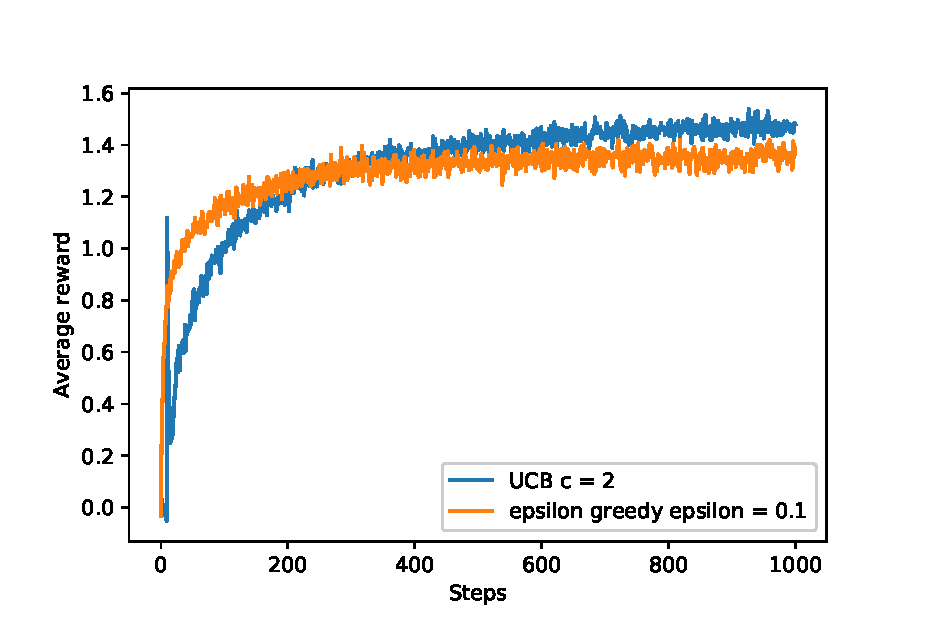
\includegraphics[width=0.6\linewidth]{Images/figure_2_4.eps}
\caption{\cite{ShangtongZhang} Learning curves of the  UCB method and the $\epsilon$-greedy method, in the first 1000 time steps.}
\label{fig:UCB}
\end{figure}

\subsection{Comparison}

	To compare the overall performance for different parameters in the given 10 armed bandit problem, a parameter study is done in Fig. \ref{fig:comparison}. For that, the learning curves are summarized by averaging over the first 1000 steps. One point in the parameter study corresponds to one learning curve.

	There are two other methods, whose performance is shown in Fig. \ref{fig:comparison}. One of them is called optimistic initialization, the other one gradient bandit. The optimistic initialization forces the agent to explore by unrealistically high initial action values, and the gradient bandit is a somewhat more complex algorithm which is studied extensively in \cite{SuttonBarto}.

	Obviously, for all four methods there are some parameter values which perform best for the task of maximizing the rewards of the first 1000 time steps. One should but always keep in mind, that for other time ranges, e.g. for 100 time steps or 10000, other parameter values may perform better. 

	The UCB method performs very well in the multiarmed bandit problem, but has difficulties with many classes of other problems, e.g. non-stationary problems. 

\begin{figure}[H]
\centering
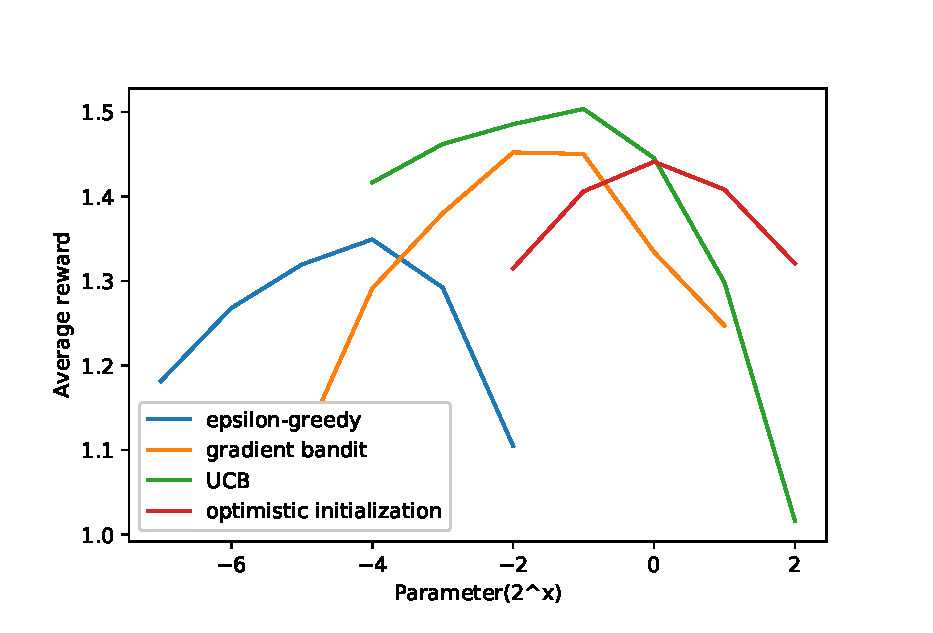
\includegraphics[width=0.6\linewidth]{Images/figure_2_6.eps}
\caption{\cite{ShangtongZhang} Parameter study of four different methods of policy learning.}
\label{fig:comparison}
\end{figure}


\section{Finite Markov Decision Processes}

	A RL problem can be generalized and put into a more rigorous framework by a Markov Decision Process. To define this, we first need to define the State-space $\mathcal{S} $, where all possible states are elements. Analogously we define the action space $\mathcal{A}$ and reward space $\mathcal{R}$. Usually all those spaces are assumed to be finite, but the theory works also for countable infinite spaces.

	Now we can define a Markov decision process as a $4$-tuple $(\mathcal{S}, \mathcal{A}, p, r)$, where
\begin{itemize}
\item $p: \begin{cases}\mathcal{S} \times \mathcal{R} \times \mathcal{S} \times \mathcal{A} \rightarrow [0,1] \\ (s',r ,s,a ) \mapsto Pr\{S_t = s', R_t = r| S_{t-1} = s, A_{t-1} = a\}  \end{cases} $ \\ is the dynamics function. It returns the probability of transitioning to state $s'$ and receiving reward $r$, when starting from state $s$ and using action $a$. \\
\item $r: \begin{cases} \mathcal{S} \times \mathcal{A} \times \mathcal{S} \rightarrow \mathcal{R} \\ (s, a, s') \mapsto r(s, a, s') \end{cases}$ \\ is the reward received after transitioning from state $s$ to state $s'$, due to action $a$.\\
\end{itemize}

	The MDP can be visualized as it is done in Fig. \ref{fig:MDP}.

\begin{figure}[H]
\centering
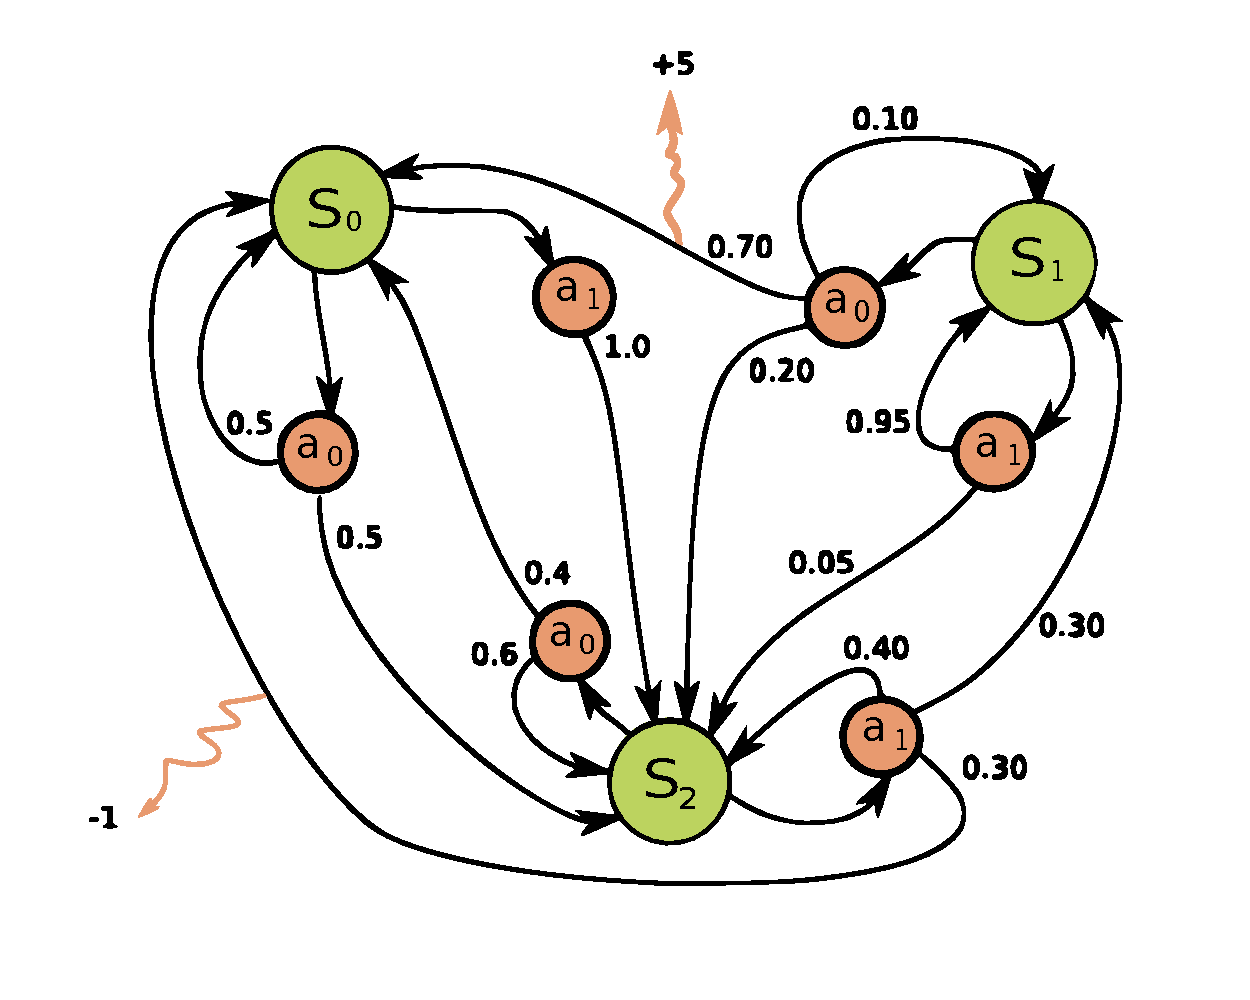
\includegraphics[width=0.6\linewidth]{Images/Markov_Decision_Process.pdf}
\caption{\cite{WikiMarkov} Visualization of a Markov Decision Process with three states, two possible actions and many different rewards, depending of the state and action.}
\label{fig:MDP}
\end{figure}

	The MDP holds two important properties: 

	The First one is called the Markov Property. It states, that in every time step the state of the MDP contains all information, that is necessary to predict future developments. So the transition probabilities or rewards do only depend on the current state and action, but not on the prior history, the states and actions that were taken before. When implementing RL problems it is always very important to check if the Markov Property is satisfied, because in complex problems some piece of necessary information is forgotten easily. 

	Second, all transition probabilities are well defined. That means, if the agent starts in a certain state and then uses a chain of certain actions, a distribution can always be calculated that tells in which state the agent might end up. In a stochastic sense, every movement is determined for given actions and beginning state. 

	These properties have an interesting implication: Given a MDP and a fixed policy, the MDP reduces to a simple Markov Chain. There are many tools to calculate Markov Chains and they are, from a mathematical point of view, relatively easy to handle. 


\subsection{Continuing Tasks}

	We required the state and action spaces to be finite, but many RL problems are in fact infinite in the time dimension. This means, they do not necessarily end after finitely many time steps. Many task that deal with control systems do only end, if the agent fails his mission. An easy example is the following one: An agent controls the engine and wheels of a cable car. The car balances an upright standing stick and the task of the agent is to control the car in such a way, that the stick keeps standing upright. If the agent succeeds in his mission, the stick will stand forever, which means for infinite time steps. Such tasks are called continuing, while tasks that end after finitely many time steps are called episodic. 

	If in this task every time step in which the stick keeps standing is rewarded with a constant value greater that zero, the expected future rewards would diverge at some point. This motivates the following definitions:

	$G_t$ is called Return at time step $t$, and is a function of the expected future rewards. In the simplest case: $G_t = R_{t+1} + R_{t+2} + R_{t+3} + ...$ This simple sum makes only sense for episodic tasks.

	For continuing tasks, the discounting factor $\gamma \in [0,1]$ is introduced. The discounting factor weights rewards that will be obtained in the far future less than rewards that will be obtained in the subsequent time steps already. The new, slightly changed, formula reads then recursively: 

\begin{align}
G_t = R_{t+1} + \gamma G_{t+1}
\end{align}

	For bounded rewards, this sum always converges.

\subsection{Bellman Equation}

	To analyze RL problems further, the following question can be asked: For a given MDP and fixed Policy, is there always a unique value function? This would enhance the value function from a convenient tool to find good policies, to an intrinsic and natural property of RL problems. And in fact, the question can be affirmed.

	Having introduced the notion of returns, the value function is the expected return when starting in $s$ and following $\pi$ thereafter:  
	 \begin{align}
	v_{\pi} (s) = \mathbb{E}\big[ G_t | S_t = s \big] = \mathbb{E}\big[ \sum_{k=0}^{\infty} \gamma^k R_{t+k+1} | S_t = s \big]
	\end{align}
The action value function is the expected return when starting in $s$, taking $a$ and following $\pi$ thereafter:  
	 \begin{align}	
	q_{\pi} (s,a) = \mathbb{E}\big[ G_t | S_t = s, A_t = a \big] = \mathbb{E}\big[ \sum_{k=0}^{\infty} \gamma^k R_{t+k+1} | S_t = s, A_t = a  \big] 
	\end{align}

	By just writing out all definitions, a recursive relation of the value function can be derived:

	\begin{align*}
	v_{\pi}(s) &= \mathbb{E} \big[ G_t | S_t = s \big] \\
	&= \mathbb{E} \big[ R_{t+1} + \gamma G_{t+1} | S_t = s \big]\\
	&= \sum_a \pi (a|s) \sum_{s'} \sum_{r} p(s',r|s,a) \big[ r + \gamma \mathbb{E} [ G_{t+1} | S_{t+1} = s' ] \big] \\
	&= \sum_a \pi(a|s) \sum_{s',r} p(s',r|s,a) \big[ r + \gamma v_{\pi}(s')  \big]
	\end{align*} 

	The result is called the Bellman Equation:

	\begin{align}
	v_{\pi}(s) = \sum_a \pi(a|s) \sum_{s',r} p(s',r|s,a) \big[ r + \gamma v_{\pi}(s')  \big] \label{bell} 
	\end{align}

	The policy $\pi$ and the dynamics function $p$ both map into the interval $[0,1]$ and can therefore be treated as constants, as well as the reward $r$ and the discounting factor $\gamma$. By keeping this in mind, one easily notices that \ref{bell} is just a system of linear equations and has therefore a unique solution. 
	
	The fact we just found can be summarized: A MDP with fixed policy has a unique value function and a recursive relation between the values of consecutive states, called the Bellman Equation. 
	
	A similar recursive relation can be derived for the action value function, as it is done in \cite{SuttonBarto}.

\subsection{Bellman Optimality Equation}

	A policy $\pi$ is better than $\pi'$ if $v_{\pi} (s) \ge v_{\pi'} (s)$ for all $s$. An optimal policy $\pi_{*}$ is better than or equal to all others. There is always at least one such.
	
	Optimal policies are sharing the same optimal action value function $q_{*}(s,a) = \max\limits_{\pi} q_{\pi} (s,a)$ for all $a,s$. This one is unique and a similar definition exists for the value function. If one chooses an optimal policy and derives the Bellman Equation, one ends up with the so called Bellman Optimality Equation:
	
	\begin{align}
	v_{*} (s) &= \max\limits_{a} \sum_{s',r} p(s',r | s,a) \big[ r + \gamma v_{*} (s') \big]\\
	q_{*} (s,a) &= \sum_{s',r} p(s',r | s,a) \big[ r + \gamma  \max\limits_{a'} q_{*} (s', a') \big] 
	\end{align}

	This produces a system of equations, which is not linear anymore and has to be implemented step wise, e.g. with dynamic programming \cite{SuttonBarto}.

\subsection{Gridworld with random and optimal policy}

	Gridworld is a game in which the agent controls a figure on a 5 times 5 grid with the possible movements up, left, right and down. When the agents moves his figure on some specific fields, it automatically jumps to another field and the agents earns a reward. If the agent bumps into a wall, he gets a reward of $-1$ and for all other moves, he gets no reward at all. The field can be seen in the left half of Fig. \ref{fig:RandomGridworld}. 
	
	At first, the game gridworld shall be played with a random policy. The agent always chooses an uniformly random action, despite his position on the field. With that policy, the value function is calculated and shown in the right half of Fig. \ref{fig:RandomGridworld}. Obviously states that are closer to the jump-and-reward states have a higher value. The value of some states close to the walls is negative, because the agent may bump into the wall more often.  

\begin{figure}[H]
\centering
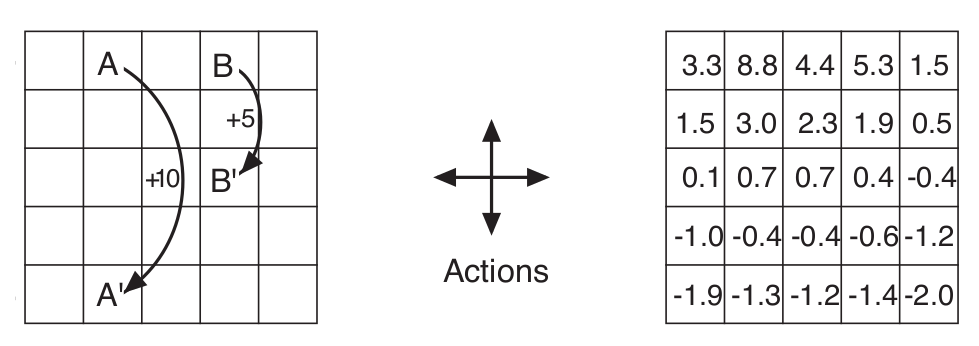
\includegraphics[width=0.6\linewidth]{Images/gridworldrandom.png}
\caption{\cite{SuttonBarto} Left: The field of gridworld. Two states are jump-and-reward states. Right: The values of the states when using a random policy.}
\label{fig:RandomGridworld}
\end{figure}

	Now the same calculations are considered, but with an optimal policy. As it can be seen in the right part of Fig. \ref{fig:OptimalGridworld}, there is more than one optimal policy. Nevertheless, all optimal policies share the same unique optimal value function, which is pictured in the middle of Fig. \ref{fig:OptimalGridworld}. The agent doesn't bump into walls anymore and therefore all the values are positive and far higher than they were before. Obviously, the returns in this example are discounted, as it is a continuing task.

\begin{figure}[H]
\centering
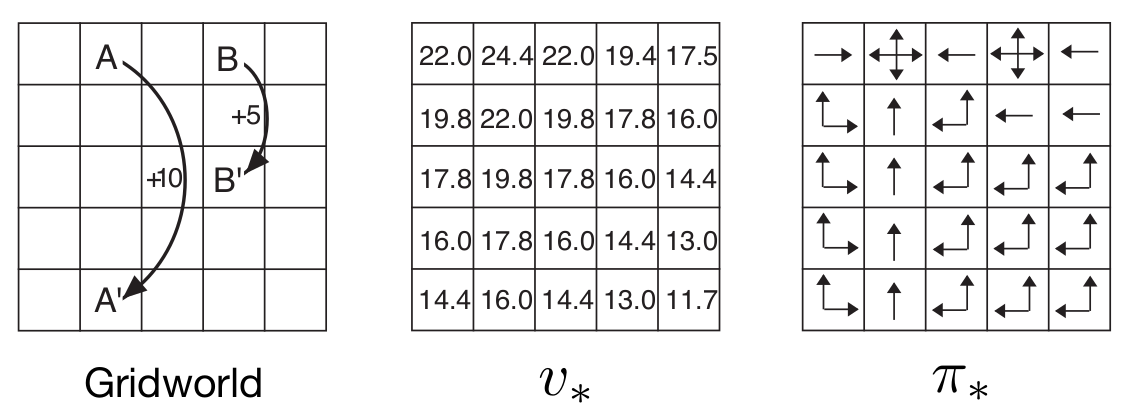
\includegraphics[width=0.6\linewidth]{Images/gridworldoptimal.png}
\caption{\cite{SuttonBarto} Gridworld with an optimal policy. This policy is not unique, as it can be seen in the right part of the picture.}
\label{fig:OptimalGridworld}
\end{figure}

\section{Project: Escape the Labyrinth}

	After establishing the theory of MDPs and calculating value functions for certain policies, an optimal policy for a generic project shall now be found. In this game, the agent has to find the fastest way out of a labyrinth, which is pictured in Fig. \ref{fig:labyrinth}. When he bumps into a wall, he gets a reward of $-1$. When he exists the labyrinth, he gets a reward of $100$. For any other action, there is no reward.

\begin{figure}[H]
\centering
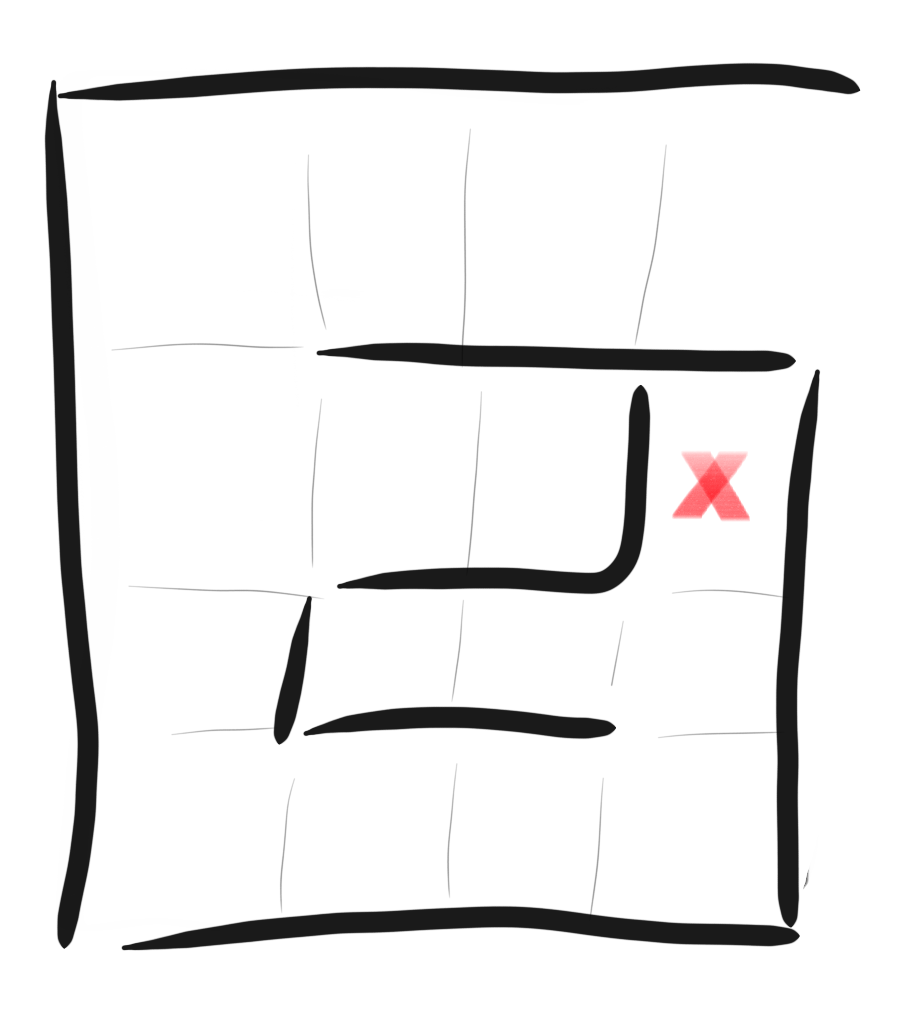
\includegraphics[width=0.2\linewidth]{Images/sketch.png}
\caption{The agent has to find the fastest way out of the labyrinth. He starts at the red cross.}
\label{fig:labyrinth}
\end{figure}

	For this task, a method called Q learning is used. At first a q-table is initialized, which contains all action values. Then the $\epsilon$-greedy method, which was discussed in chapter 2, is applied. After every greedy move, the q table is updated with the following update rule: 
	
\begin {align}
q(s_t,a_t) \leftarrow (1 - \alpha) q(s_t,a_t) + \alpha[R(s_t,a_t) + \gamma \max\limits_a q(s_{t+1},a)]
\end{align}

	Here $\alpha \in [0,1]$ is the learning rate and $\gamma \in [0,1]$ the discounting factor. The similarity of the update rule to the bellman equation can be noticed easily. The update rule is in fact a step wise implementation of the bellman equation.

\subsection{Results}

	For the implementation, the parameters $\gamma = 0.7$ and $\alpha = 0.5$ worked best. $\epsilon$ was linearly decreased over the learning process, such that it started by 1 and ended by 0. The best result, that could be obtained, was finding an optimal policy after 30 episodes. In this case one episode starts with the agent at the start position and ends when he exists the labyrinth. With an optimal policy, the agent should only need 11 steps. As it can be seen in \ref{fig:LabLearning}, the agent needs many more steps in the beginning. The degree of exploration is in the beginning still very high, as $\epsilon$ is close to $1$. 

\begin{figure}[H]
\centering
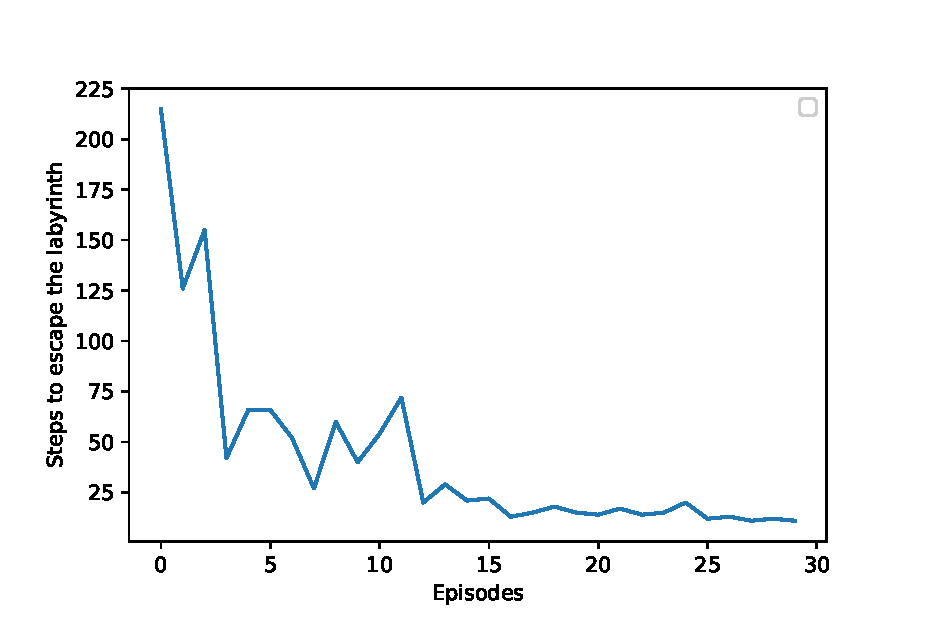
\includegraphics[width=0.6\linewidth]{Images/learning_curve.eps}
\caption{Learning curve of the agent in the labyrinth escape. After 30 episodes an optimal policy is found, which enables the agent to exit the labyrinth with 11 steps.}
\label{fig:LabLearning}
\end{figure}

When the agent has found the optimal policy, the q table shows higher values the closer the agent gets to the exit. It can be seen in Fig. \ref{fig:LearnedQTables}. In \ref{fig:OptimalAction} the optimal action to leave the labyrinth in the most direct way is shown.

\begin{figure}[H]
\centering
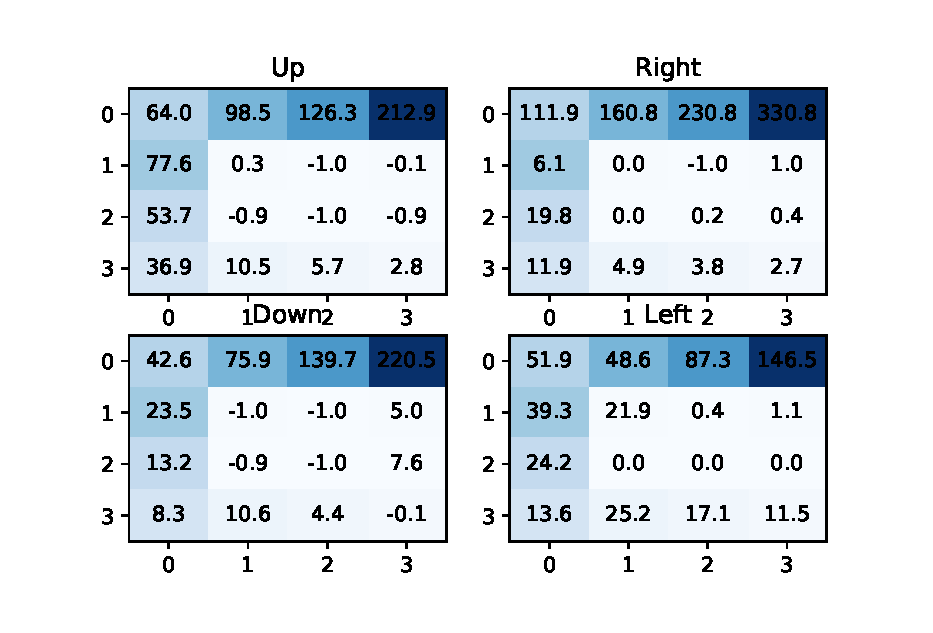
\includegraphics[width=0.7\linewidth]{Images/direction_values.eps}
\caption{Learned q-table with the optimal policy.}
\label{fig:LearnedQTables}
\end{figure}

\begin{figure}[H]
\centering
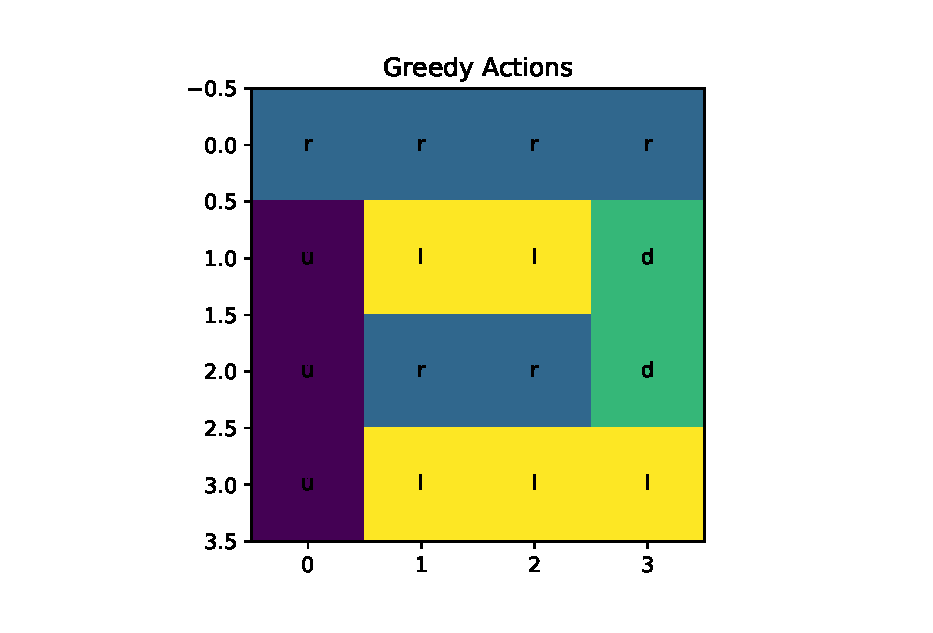
\includegraphics[width=0.6\linewidth]{Images/greedy_directions.eps}
\caption{Optimal Actions from every state, to leave the labyrinth on the most direct way.}
\label{fig:OptimalAction}
\end{figure}

\subsection{Discussion}

	The Labyrinth problem could be solved, using Q Learning. It had to be expected, that the agent would need some episodes to find the optimal policy. The learning process could maybe be speeded up by different rewards: Penalizing every time step, which does not lead to the exit instead of only penalizing bumps into the walls would probably prevent the agent from loosing too many steps in the area close to the starting point. Anyway, the rewards were chosen in that way to model a real person, which is searching for an exit of the labyrinth, most realistically. 
	
	The discounting factor had to be chosen very high, which is typical for RL problems with positive rewards that only come at the very end of the game. If the discounting factor was too small, the agent would only see the reward when he is close to the end already.

%----------------------------------------------------------------------------------------

\bibliographystyle{plain}
\bibliography{wagner}

\end{document}
